\section{Abstract}

Low temperature reactions between laser-cooled \ce{Be+(^2S1/2)} ions and partially deuterated water (\ce{HOD}) molecules have been investigated using an ion trap and interpreted with zero-point corrected quasi-classical trajectory calculations on a highly accurate global potential energy surface for the ground electronic state. Both product channels have been observed for the first time, and the branching to \ce{BeOD+ + H} is found to be $0.58 \pm 0.14$. The experimental observation is reproduced by both quasi-classical trajectory and statistical calculations. Theoretical analyses reveal that the branching to the two product channels is largely due to the availability of open states in each channel.

\section{Introduction}

Together, isotope substitution and the measurement of the resulting product branching ratios provide important details about reaction dynamics and are often used to identify reaction pathways and understand bond-selective chemistry.\cite{Crim1990,Crim1996,Zare1998} Important examples include X + HOD (X = H, F, Cl, O) reactions, where the branching ratios are experimentally controlled by selective excitation of the O–H or O–D bond.\cite{Sinha1990,Bronikowski1991,Metz1993a,Zhang1997,Song2015,Song2015a,Fu2015,Zheng2018a,Skouteris1999b} It is now understood that a highly-accurate potential energy surface (PES) is crucial for performing theoretical calculations of the product branching ratio, where subtle, difficult to identify, PES features have been found to significantly affect the results.\cite{Skouteris1999b}

A sophisticated understanding of radical-molecule reaction dynamics is continuing to develop from extensive experimental and theoretical studies. However, despite their importance in interstellar chemistry, where the isotopic branching ratios strongly influence the products of the interstellar cloud chemical network,\todo{14} far less progress has been made in the study of ion–molecule reactions at low temperature. This is largely due to the challenges associated with both the experimental and theoretical approaches to these systems.\cite{Clary1990,Dateo1989,Adams1976,Armentrout2002,Sims2002,Smith2000,Snow2008} Experimental difficulties include a lack of quantum state preparation and readout techniques, while theoretical difficulties appear when treating dynamics dominated by the long range interaction between ions and molecules. Recently, several groups have employed cold (~mK) and fully-controlled laser-cooled trapped ions to address these experimental issues. For instance, isotope selectivity was probed in the reaction of laser-cooled Mg+ with HD,\todo{22} and the formation rate of \ce{MgD+} was found to be 5 times greater than \ce{MgH+}. This observation was ascribed to a dynamic mechanism in the exit channel of the reaction since statistical methods predict only a factor of approximately 2.\cite{Dalleska2005} A similar experimental technique was applied to \ce{Ca+ + HD} reactions as well,\cite{Hansen2012} where the \ce{CaD+} channel was found to have ~1.5 times higher population than the \ce{CaH+} channel; no detailed theoretical calculations have been performed for this system. With the help of laser-cooled ions, the initial quantum states are experimentally well controlled, but highly accurate PESs are still challenging to calculate with \ce{Mg+} or \ce{Ca+} ions due to the complexity of their electronic structures. The development of a more comprehensive understanding of ion–molecule reactions at low temperature will benefit from studies with less complex species that are amenable to theoretical treatment.

In this publication, we report a combined experimental and theoretical study of the effect of isotope substitution in an ion–polyatomic molecule reaction. A key objective is to understand the role of dynamics in such a reaction. Previous work on Be+ + H2O showed that chemical dynamics resulting from a submerged barrier strongly affect the reaction, leading to a reduction of the overall reaction rate from the capture limit. The overestimation by the capture model was thus taken as a sign that this reaction is not completely statistical, despite the existence of a deep BeH2O+ potential well along the reaction path. In this work, we probe the dynamics by examining the product branching ratio, which is presumably controlled by the exit channel barriers. Such a measurement is much more sensitive to the determination of the overall rates. Interestingly,
here we find that the measured deuteration fraction of the ionic products is in good agreement with quasi-classical trajectory (QCT) calculations on the ground state PES. Furthermore, the branching ratio can be explained by a statistical model based on complete energy randomization in the long-lived transition complex.

\section{Experimental}

The apparatus employed here has been described in detail elsewhere. Briefly, laser ablation of metallic \ce{Be} is used to produce \ce{Be+} ions, which are trapped in a linear radio frequency Paul trap. Laser cooling\cite{Wineland1979} is used to cool the translational motion of the ions, resulting in a Coulomb crystal of Be+ ions. A time-of-flight mass spectrometer (TOF-MS)\cite{Schowalter2012,Schneider2014,Puri2017,Paul1990} is integrated into the Paul trap to analyze reaction products, allowing investigation of the isotope effect by mass spectrometry of the trapped ionic products. The 313 nm laser for cooling \ce{Be+} ions allows manipulation of the Be+ electronic quantum states; by tuning the frequency of this cooling laser, the fraction of ions in the \ce{^2S1/2} and \ce{^2P3/2} states can be precisely controlled. Promotion of the Be+ to the \ce{^2P3/2} state opens more product pathways, as well as modifies existing product channels. HOD is made by mixing \ce{H2O} and \ce{D2O}.\cite{Pyper1967,Zhou2013} The gaseous room-temperature \ce{HOD/H2O/D2O} mixture is then introduced
via a leak valve into the trapping region for reaction with the trapped ions, the actual ratio of the mixture is measured from a Stanford Research Systems (SRS) residual gas analyzer (RGA). The RGA’s fractionation of water was calibrated by introducing the water vapor into the chamber and integrating all resulting m/z signals.
A typical scan reveals water fractionation products at $m/z =$ 18, 17, and 16, which coincide with \ce{H2O+}, \ce{OH+}, and \ce{O+}. The fractionation ratios of water are found by solving the system of equations:

\begin{align}
	P_{\ce{H2O}} & = R_{18} + R_{17} + R_{16} \\
	R_{18} & = \alpha P_{\ce{H2O}} \\
	R_{17} & = \beta P_{\ce{H2O}} \\
	R_{16} & = \gamma P_{\ce{H2O}}
\end{align}

where $R_i$ is the pressure reading from the RGA and $P_{\ce{H2O}}$ is the true \ce{H2O} pressure. These fragmentation ratios were found to be $\alpha = 0.768 \pm 0.006$, $\beta = 0.184 \pm 0.006$ and $\gamma = 0.068 \pm 0.002$. The
direct readings from analog scans with deuterated samples were then adjusted to account for the fractionation for each isotopologue.

\begin{align}
	P_{\ce{H2O}} & = \frac{1}{\alpha}\left(R_{18} - \frac{\beta}{\alpha}R_{20} - \frac{\beta}{2\alpha} R_{19}\right) \\
	P_{\ce{HOD}} & = \frac{R_{19}}{\alpha} \\
	P_{\ce{D2O}} & = \frac{R_{20}}{\alpha}
\end{align}

\begin{figure}[H]
	\centering
	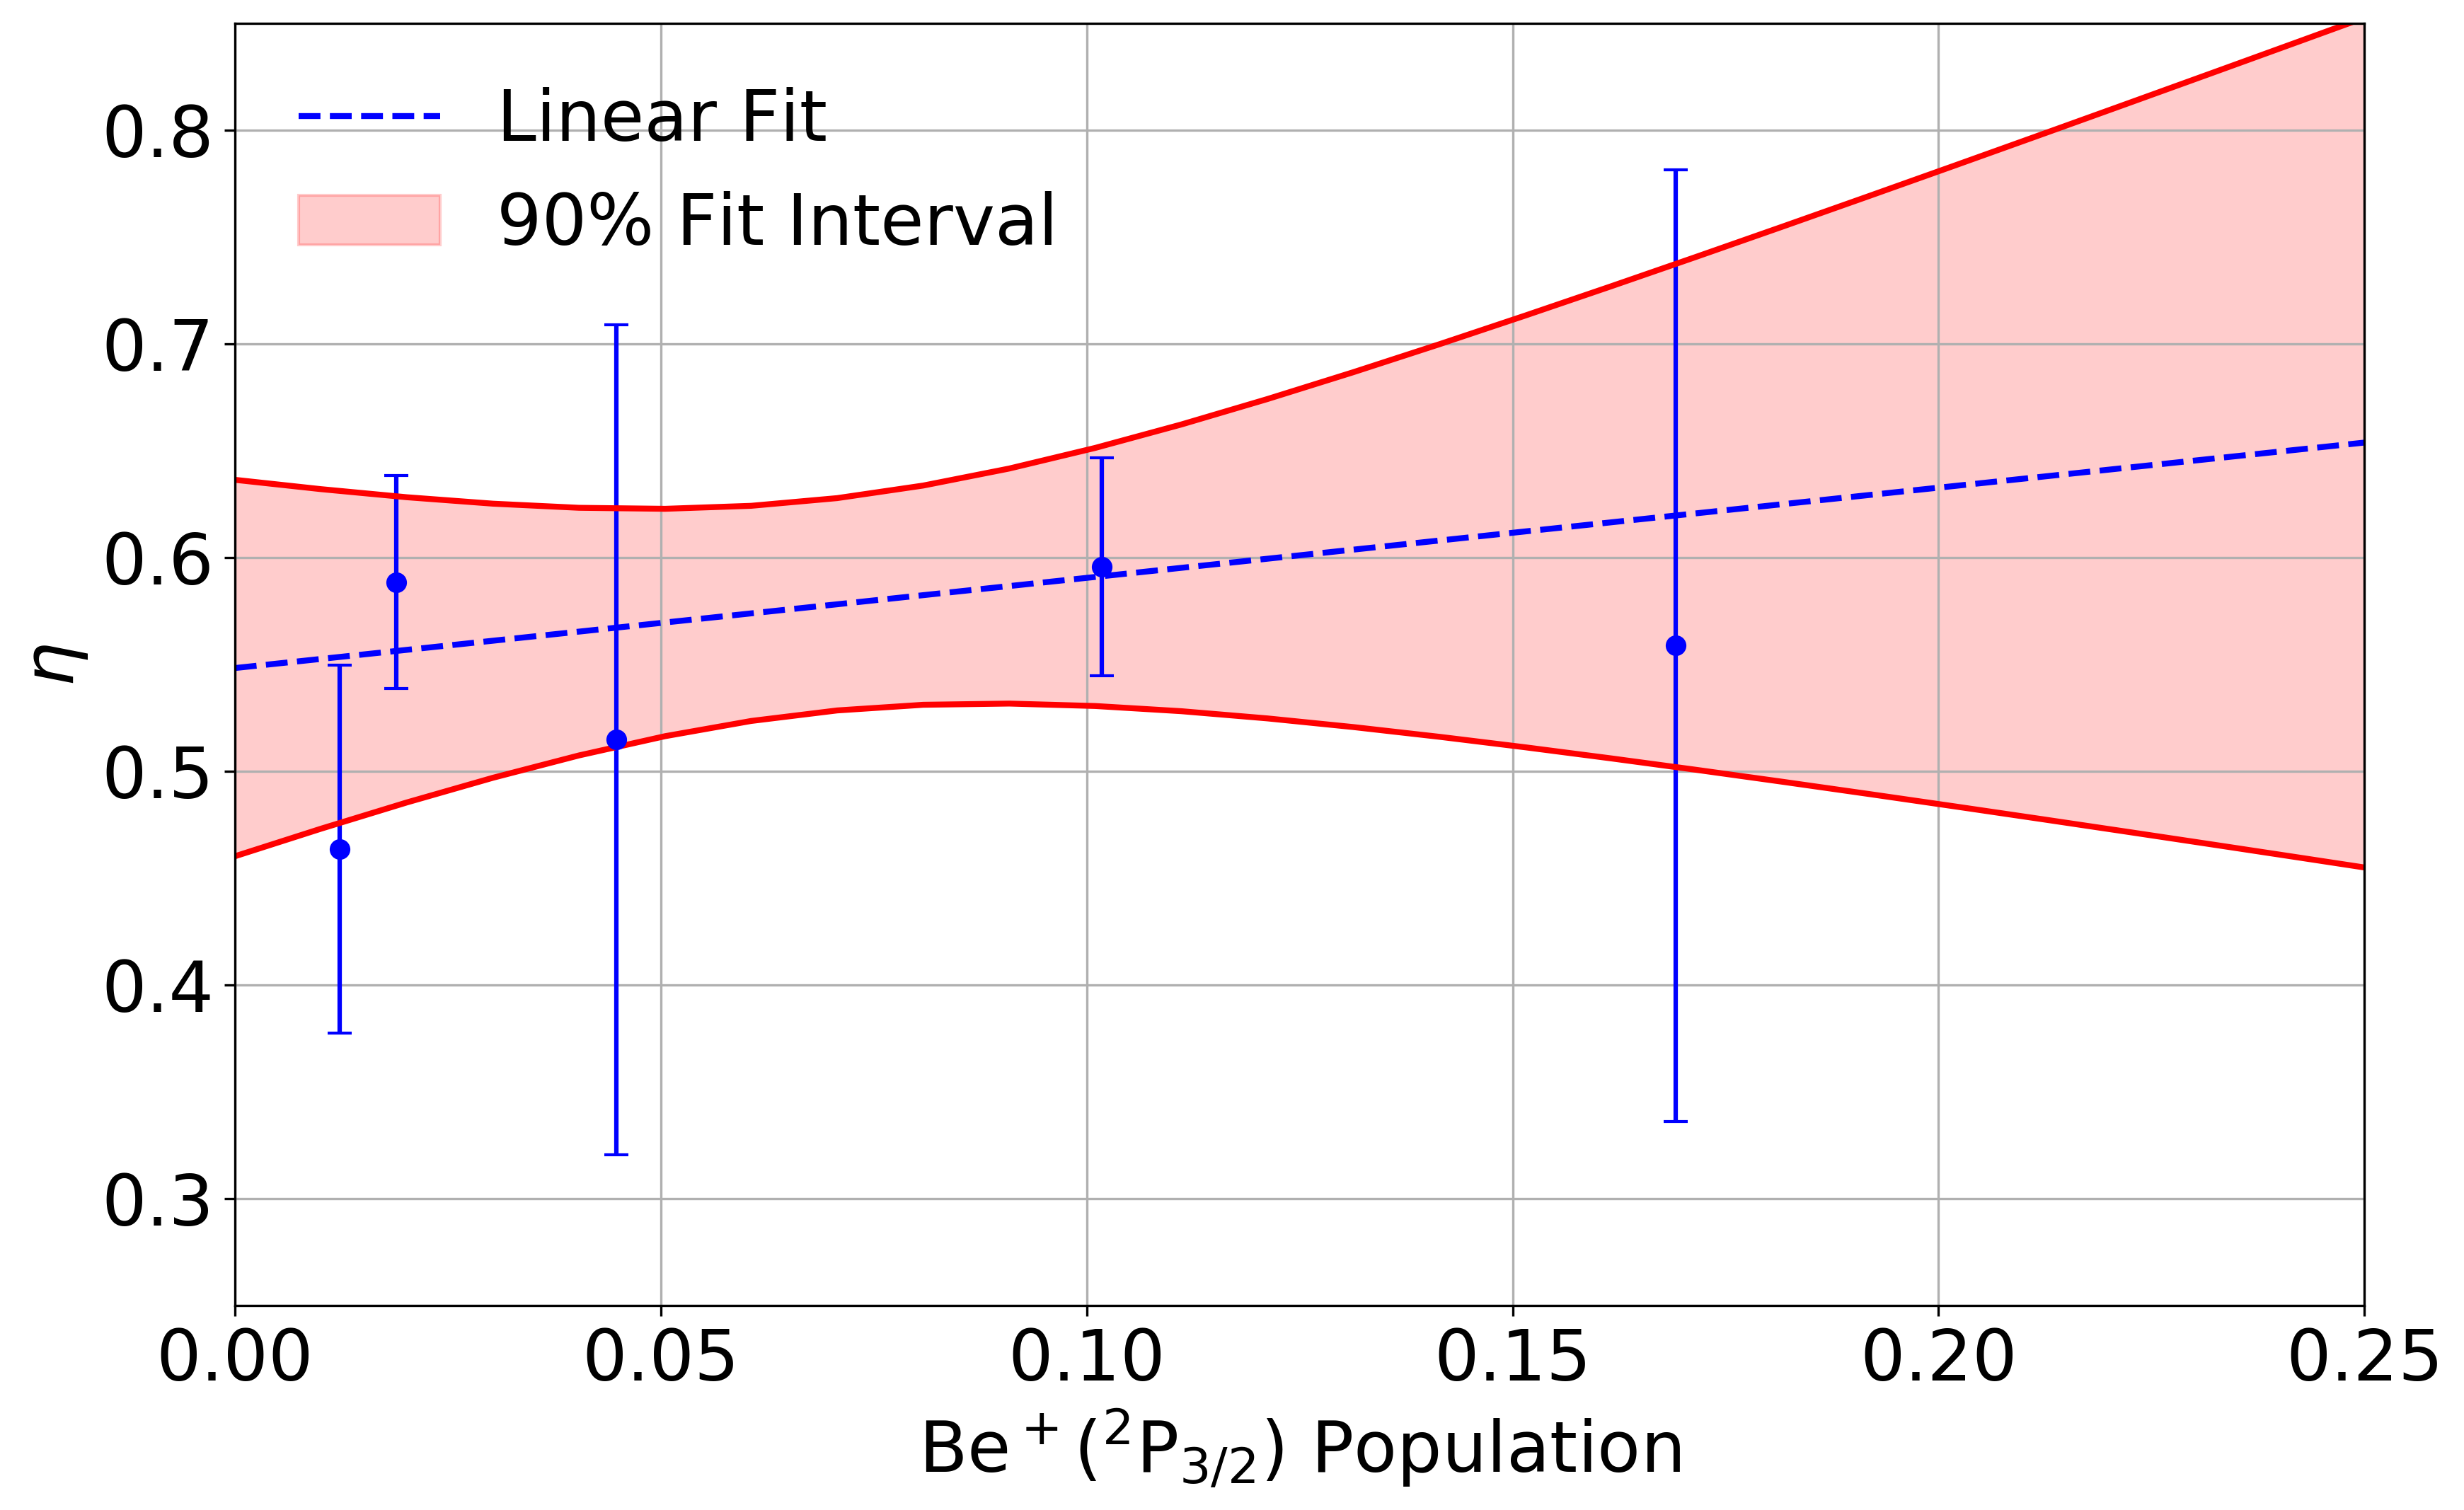
\includegraphics[width=0.8\textwidth]{images/Be_HOD_p_state.png}
	\caption{}
	\label{}
\end{figure}

\begin{figure}[H]
	\centering
	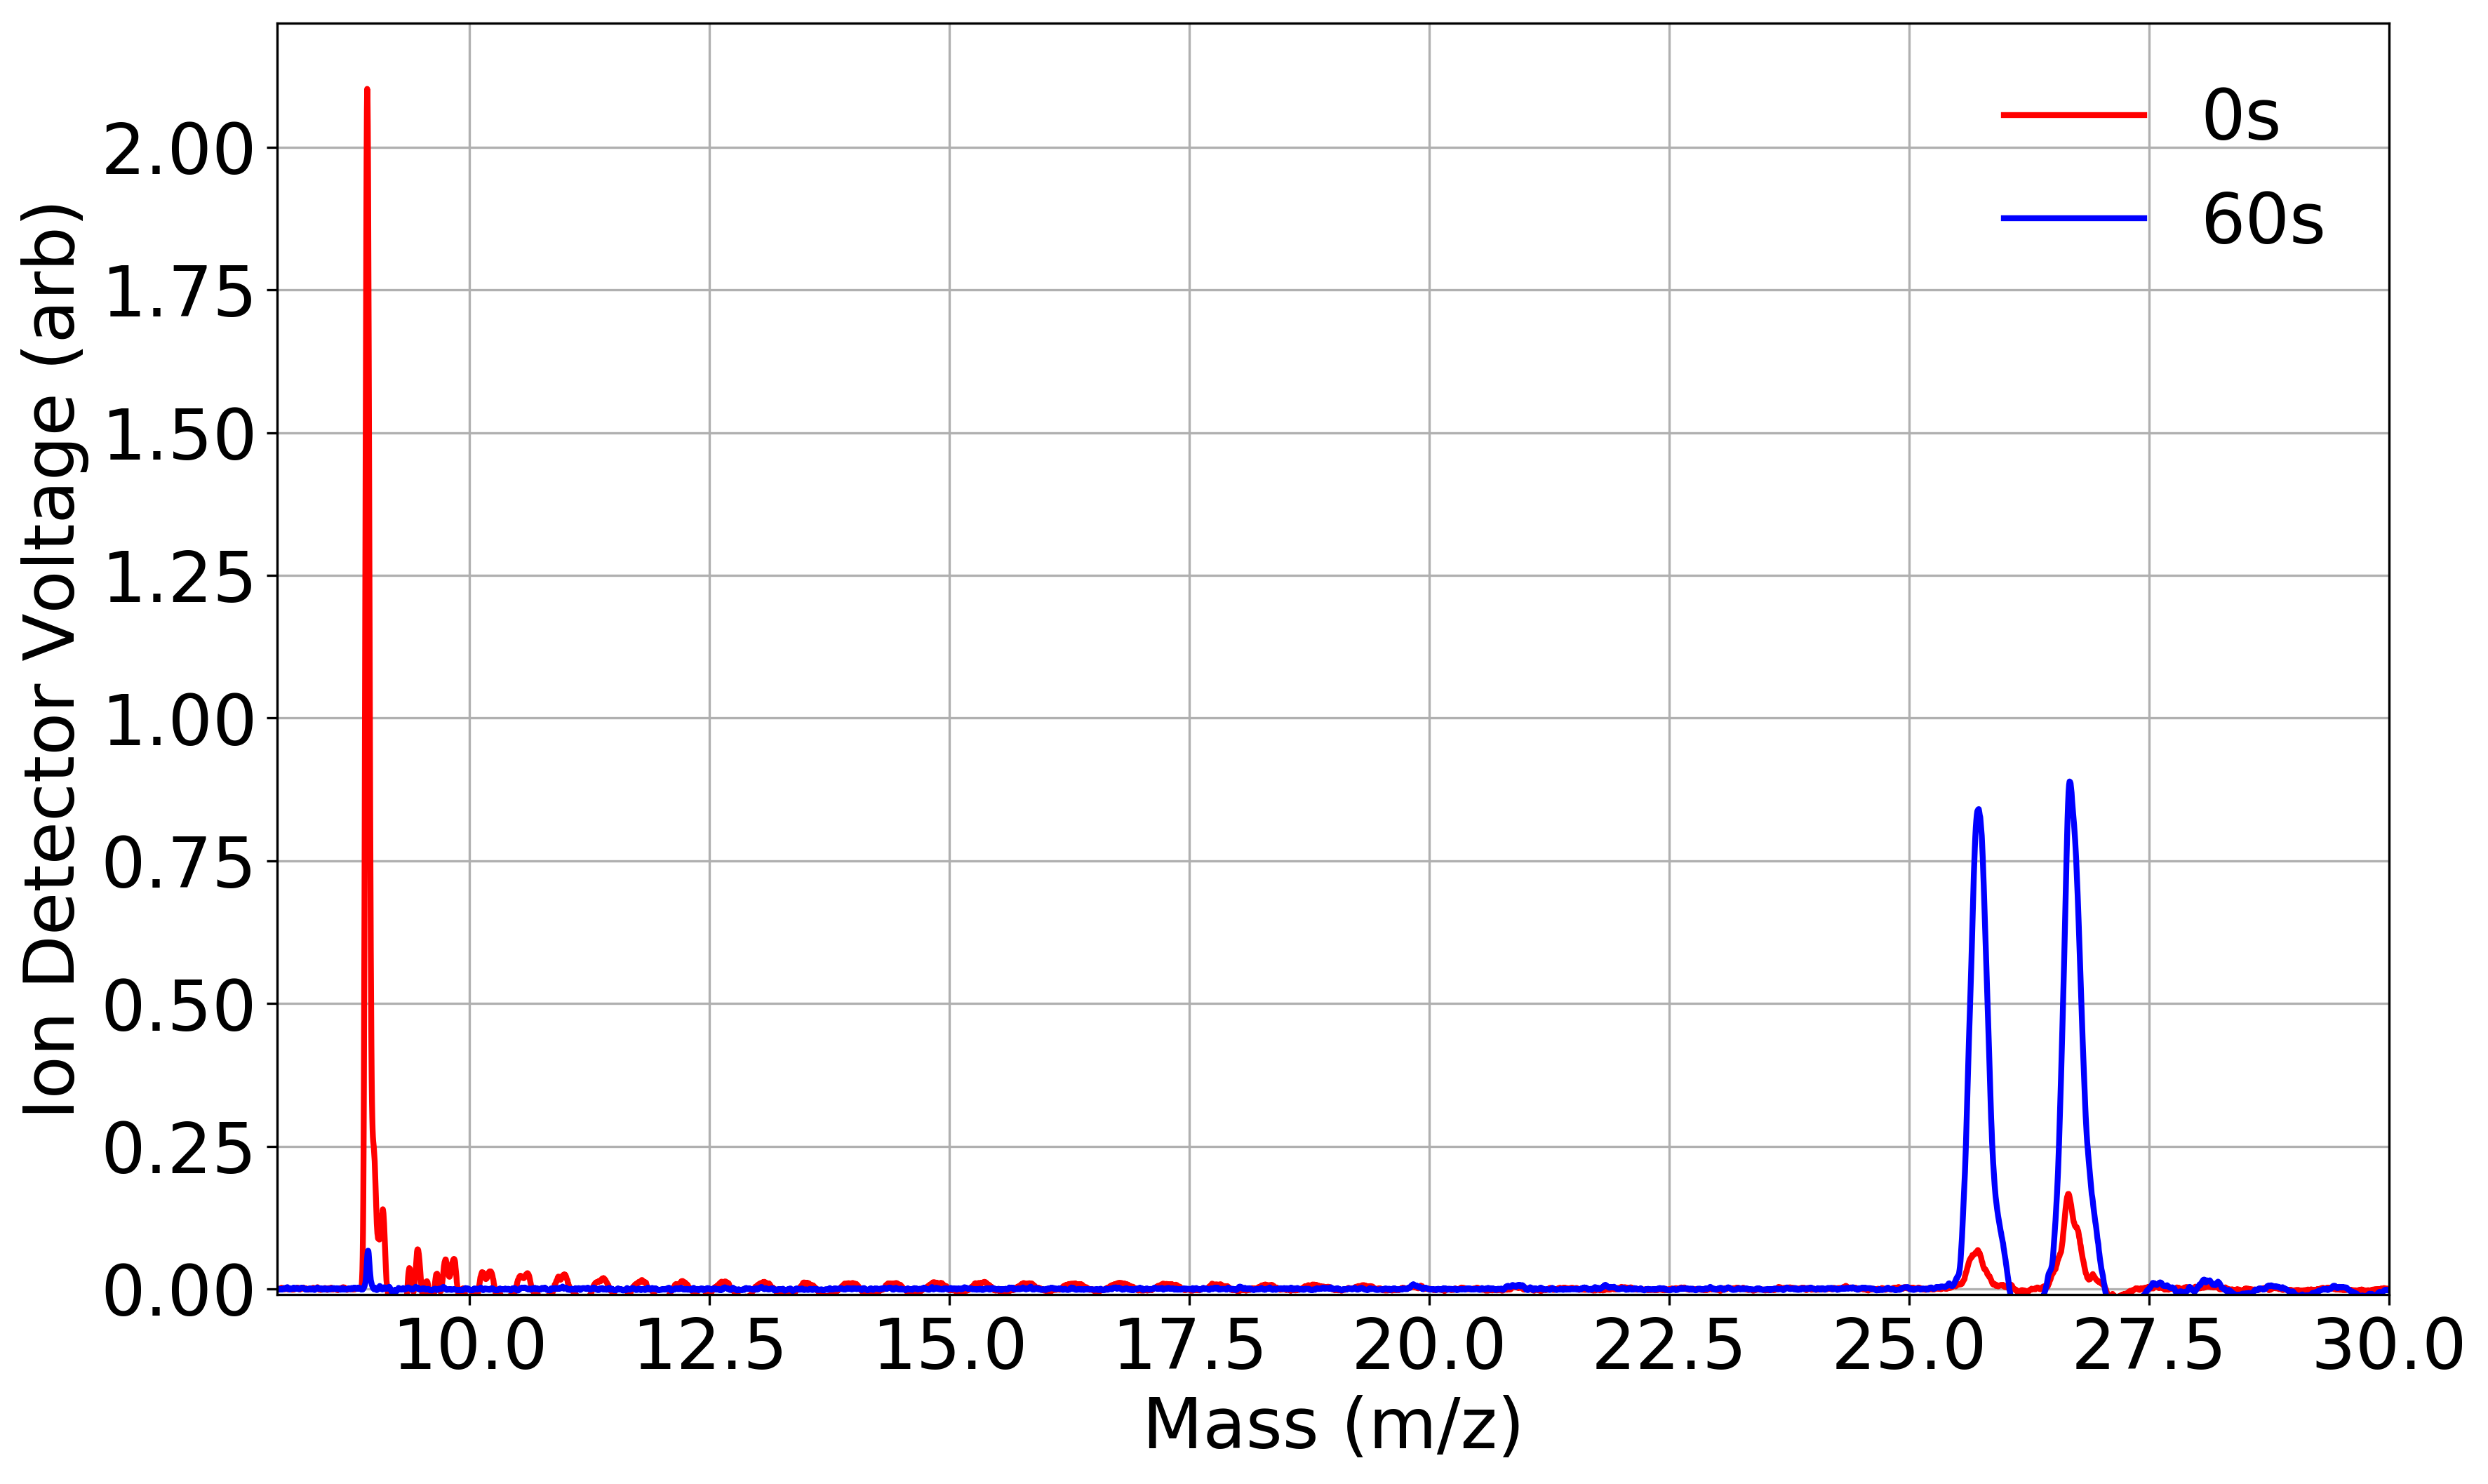
\includegraphics[width=0.8\textwidth]{images/Be_HOD_TOF.png}
	\caption{}
	\label{}
\end{figure}

\begin{figure}[H]
	\centering
	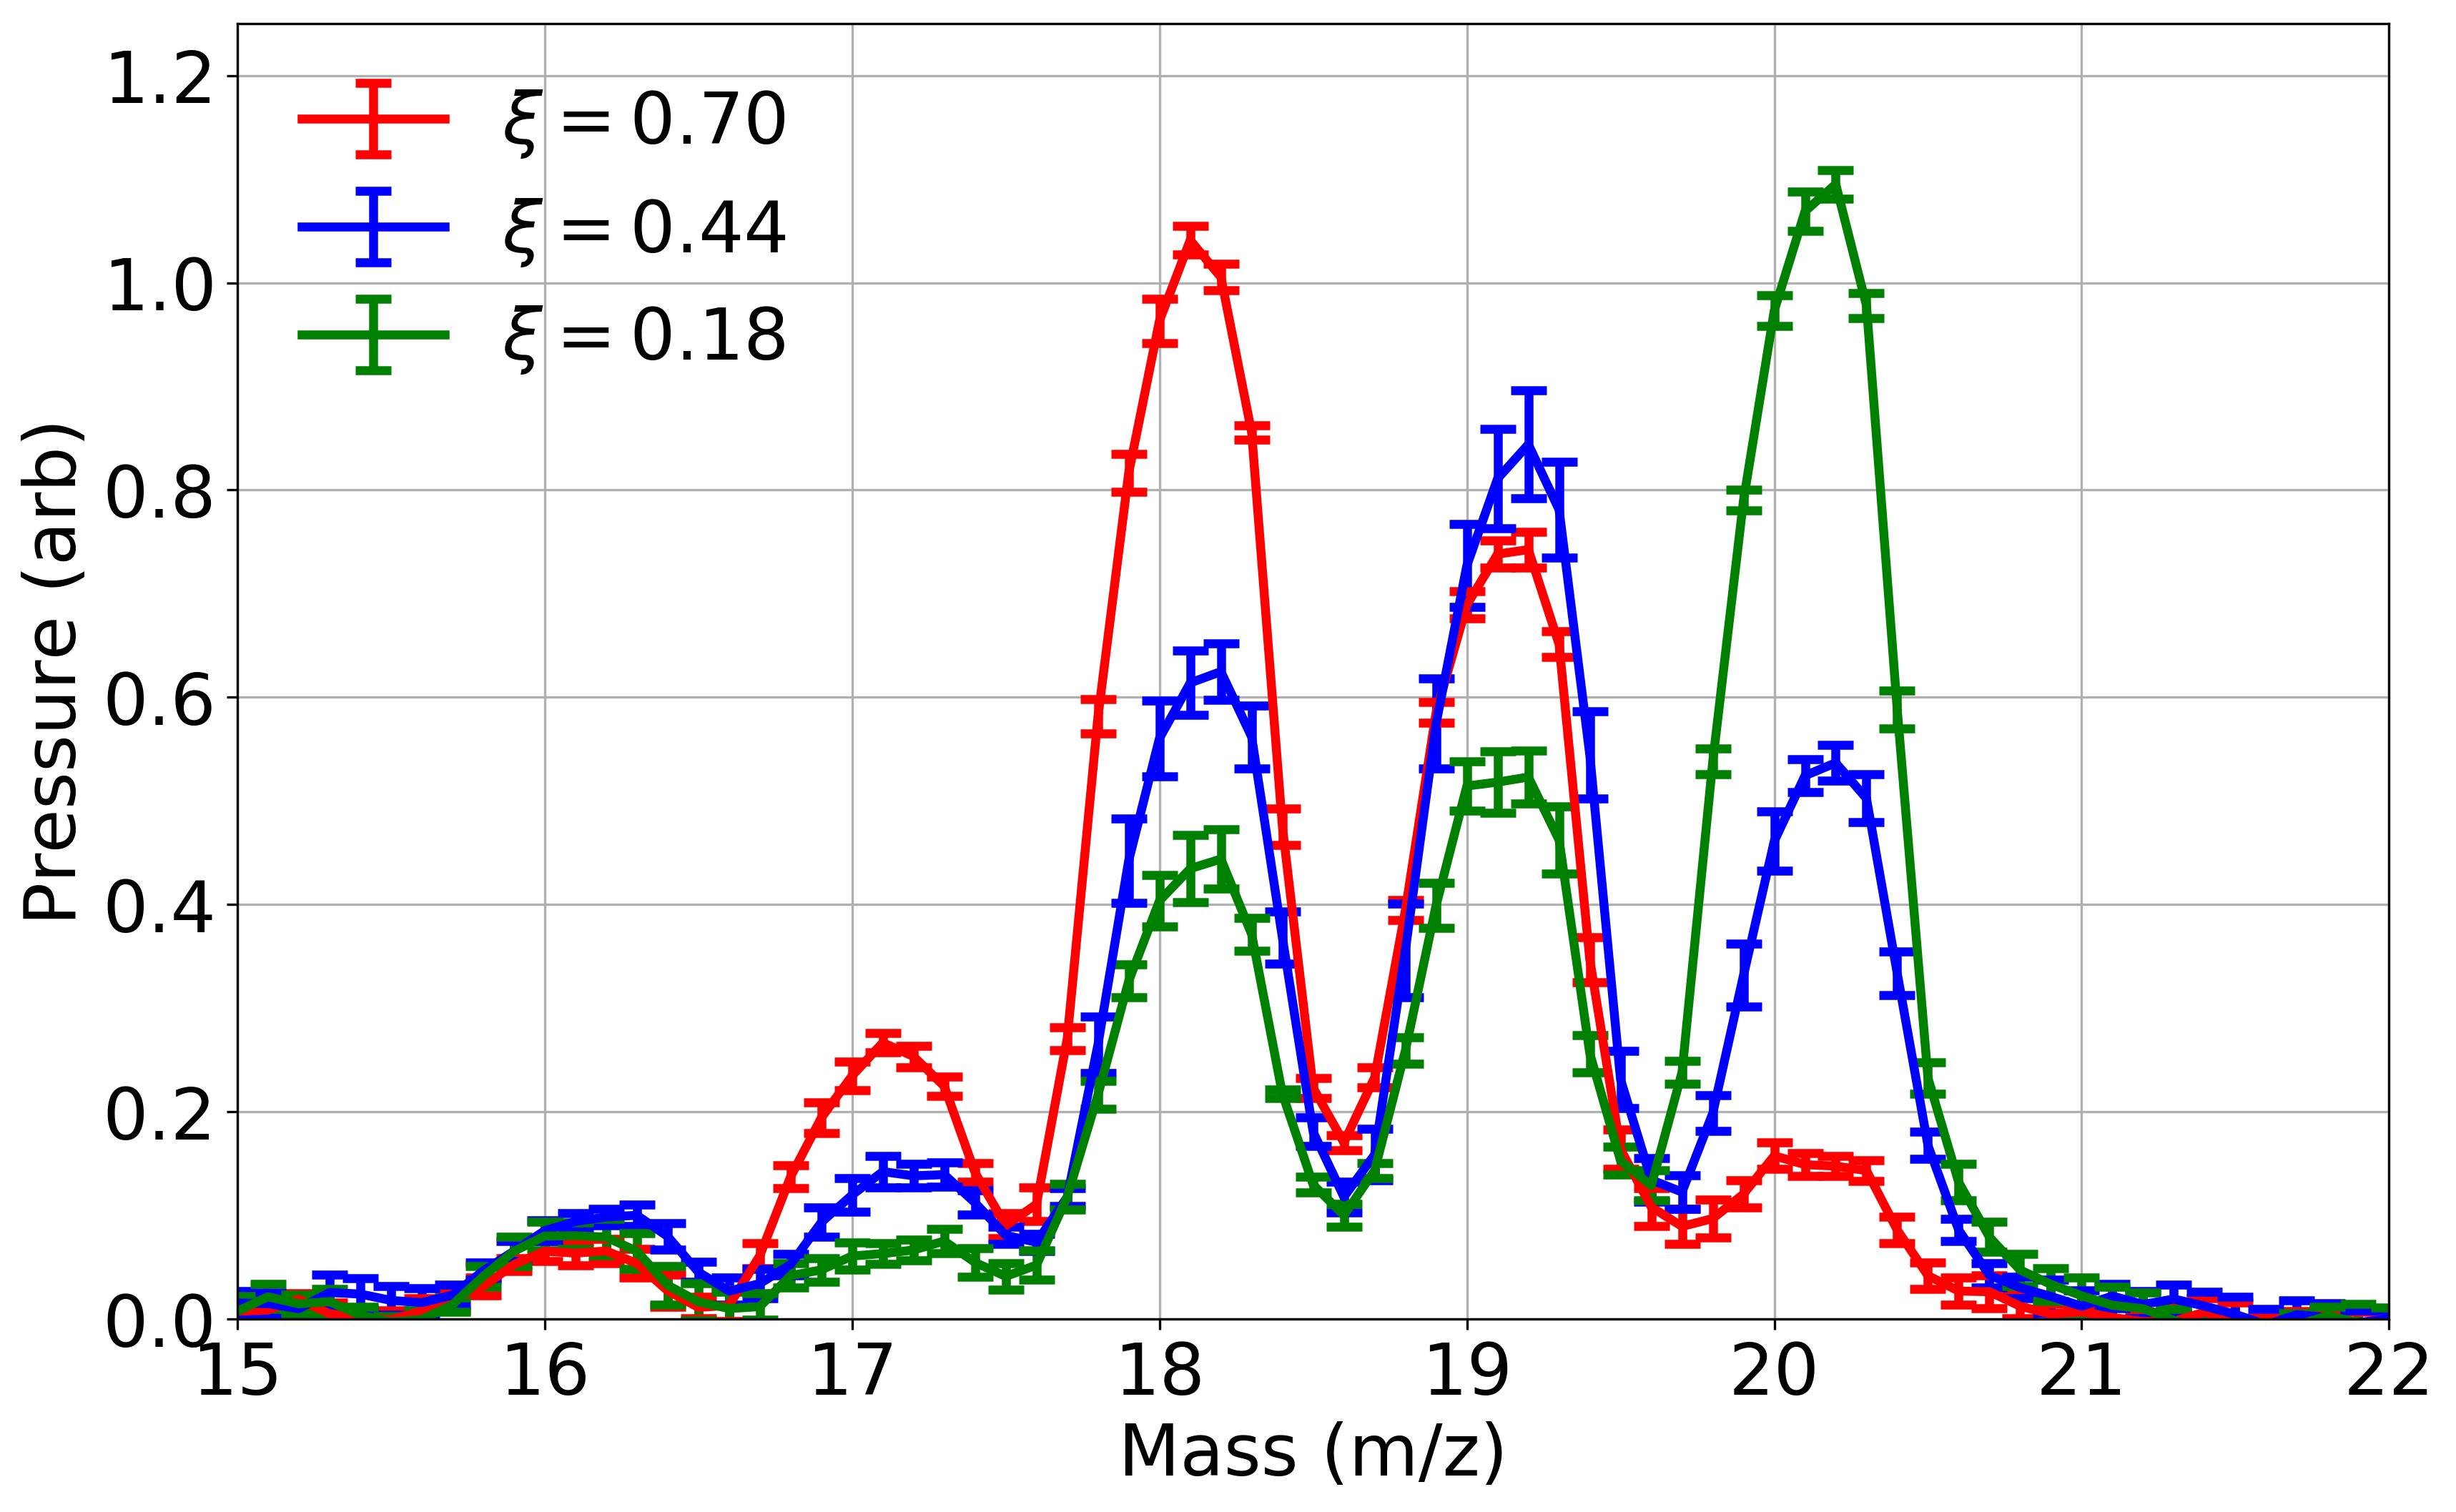
\includegraphics[width=0.8\textwidth]{images/Be_HOD_RGA.png}
	\caption{}
	\label{}
\end{figure}

\begin{figure}[H]
	\centering
	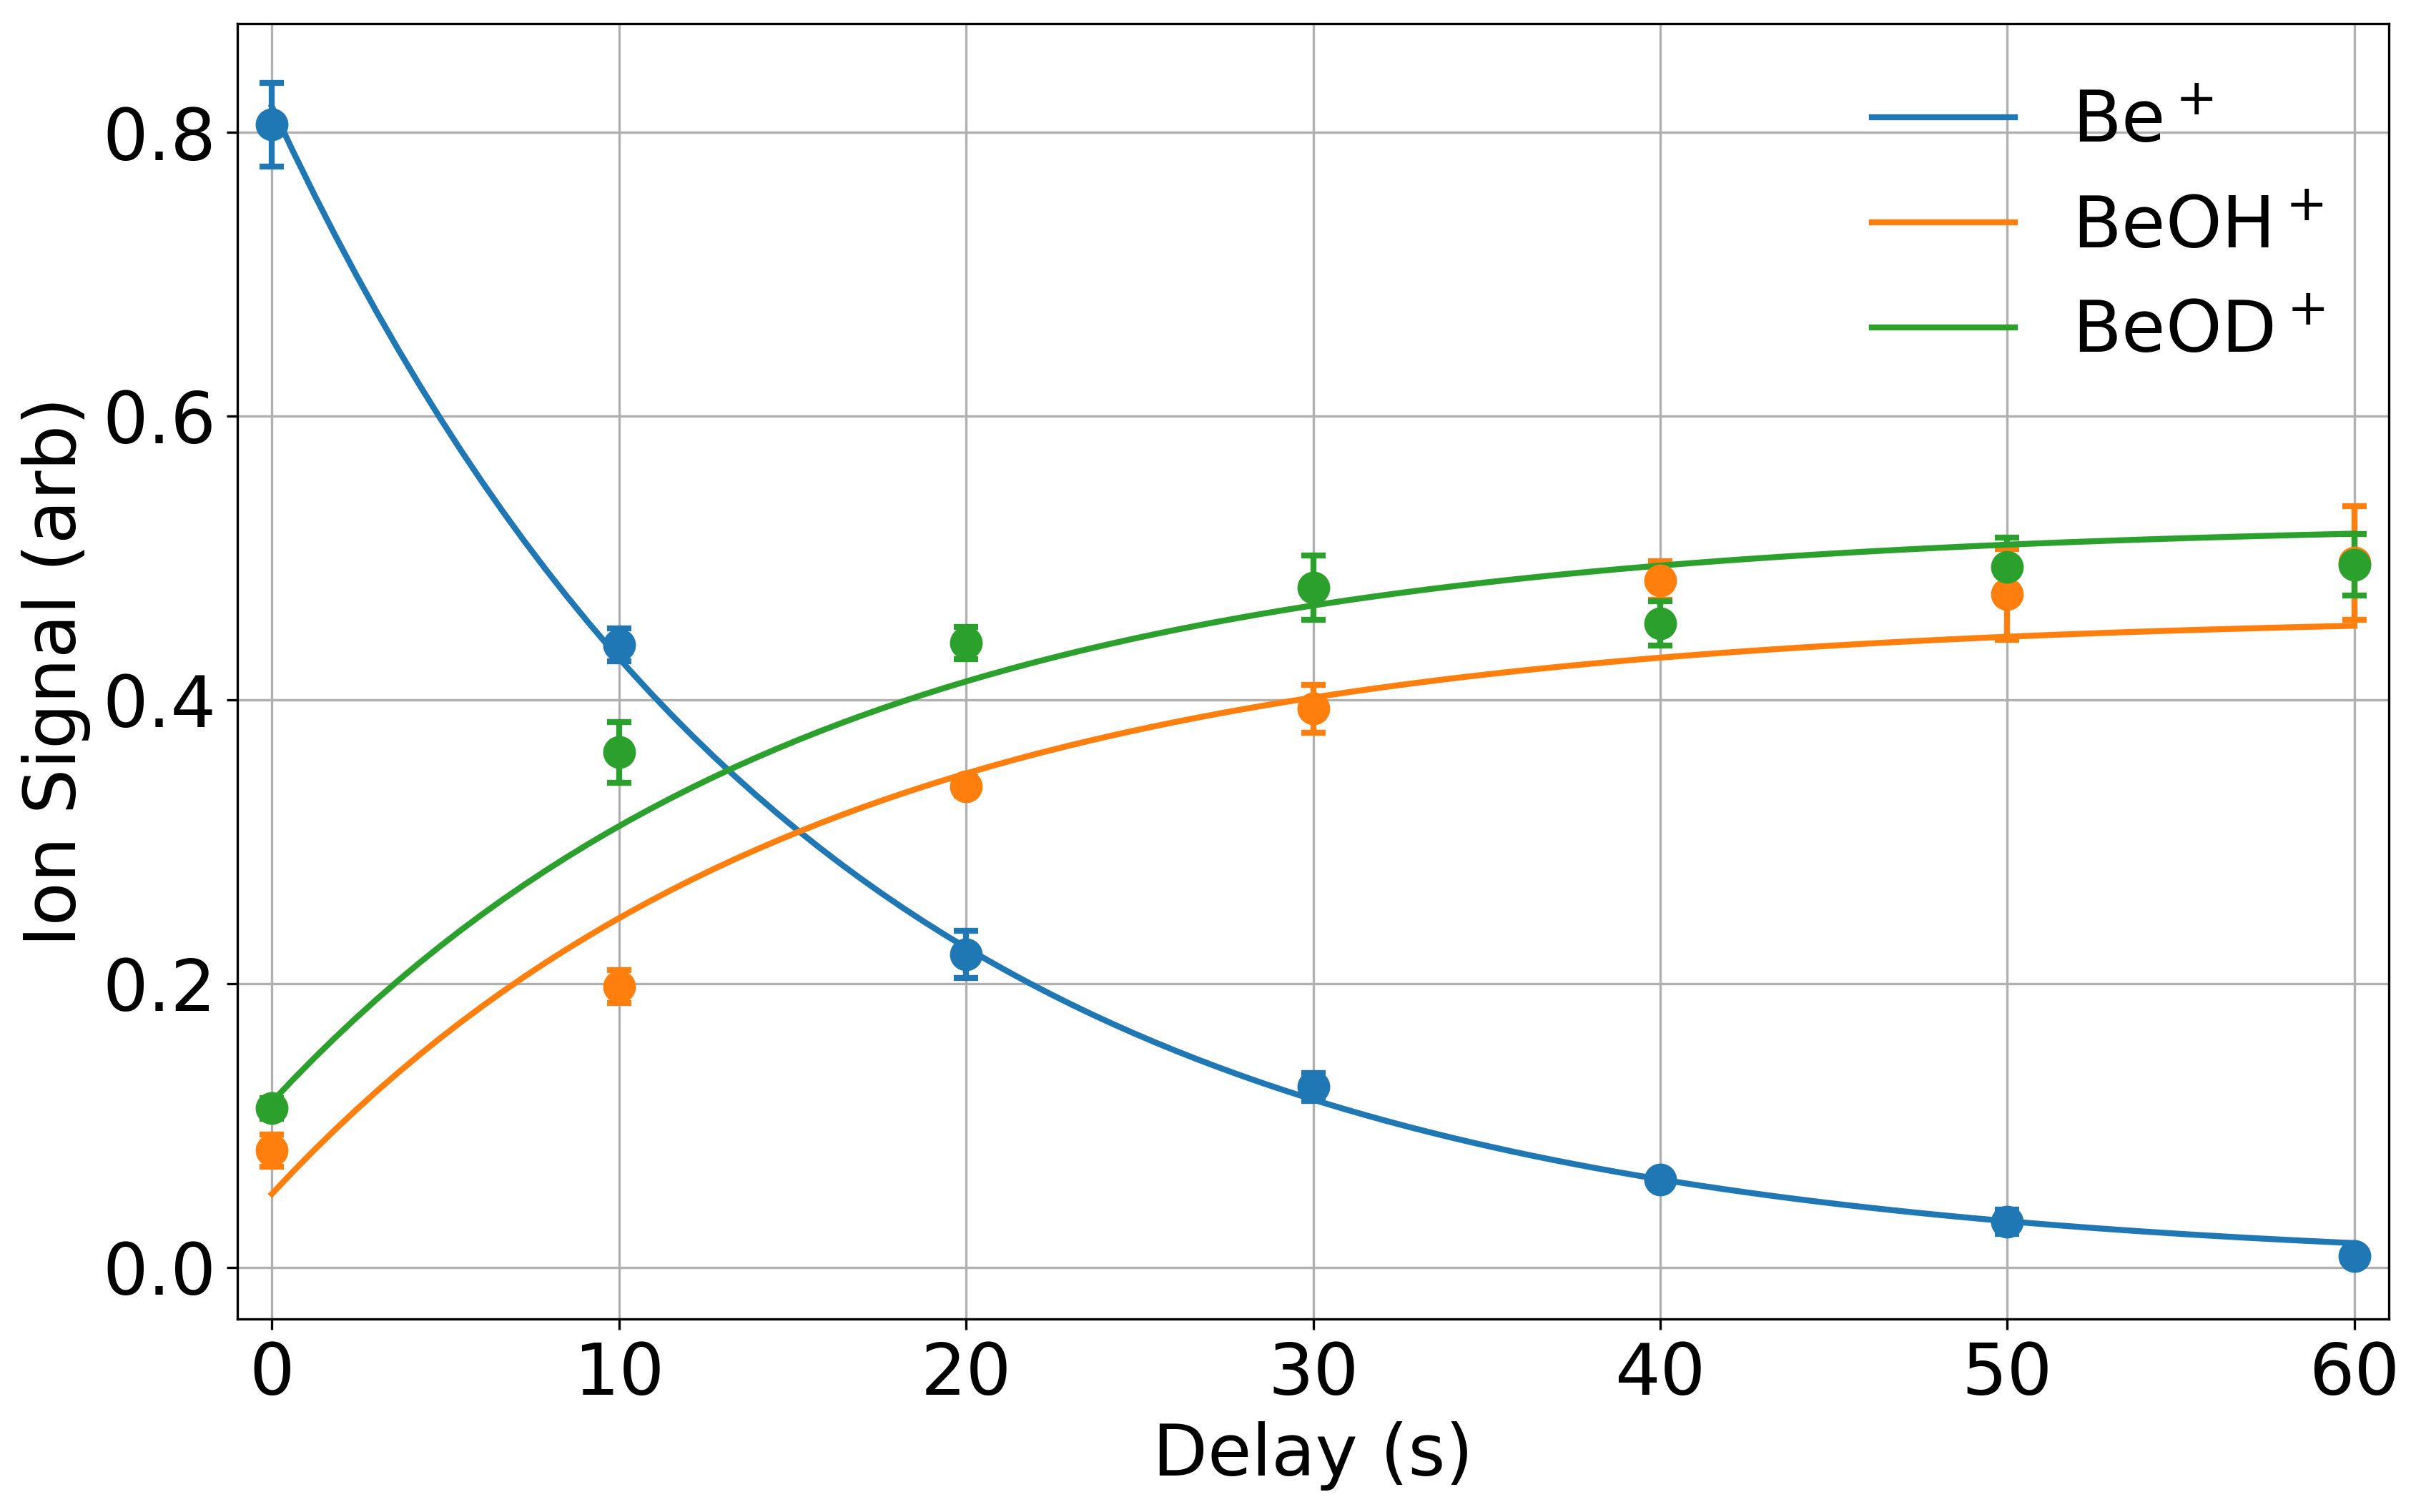
\includegraphics[width=0.8\textwidth]{images/Be_HOD_shared_fit.png}
	\caption{}
	\label{}
\end{figure}

\begin{figure}[H]
	\centering
	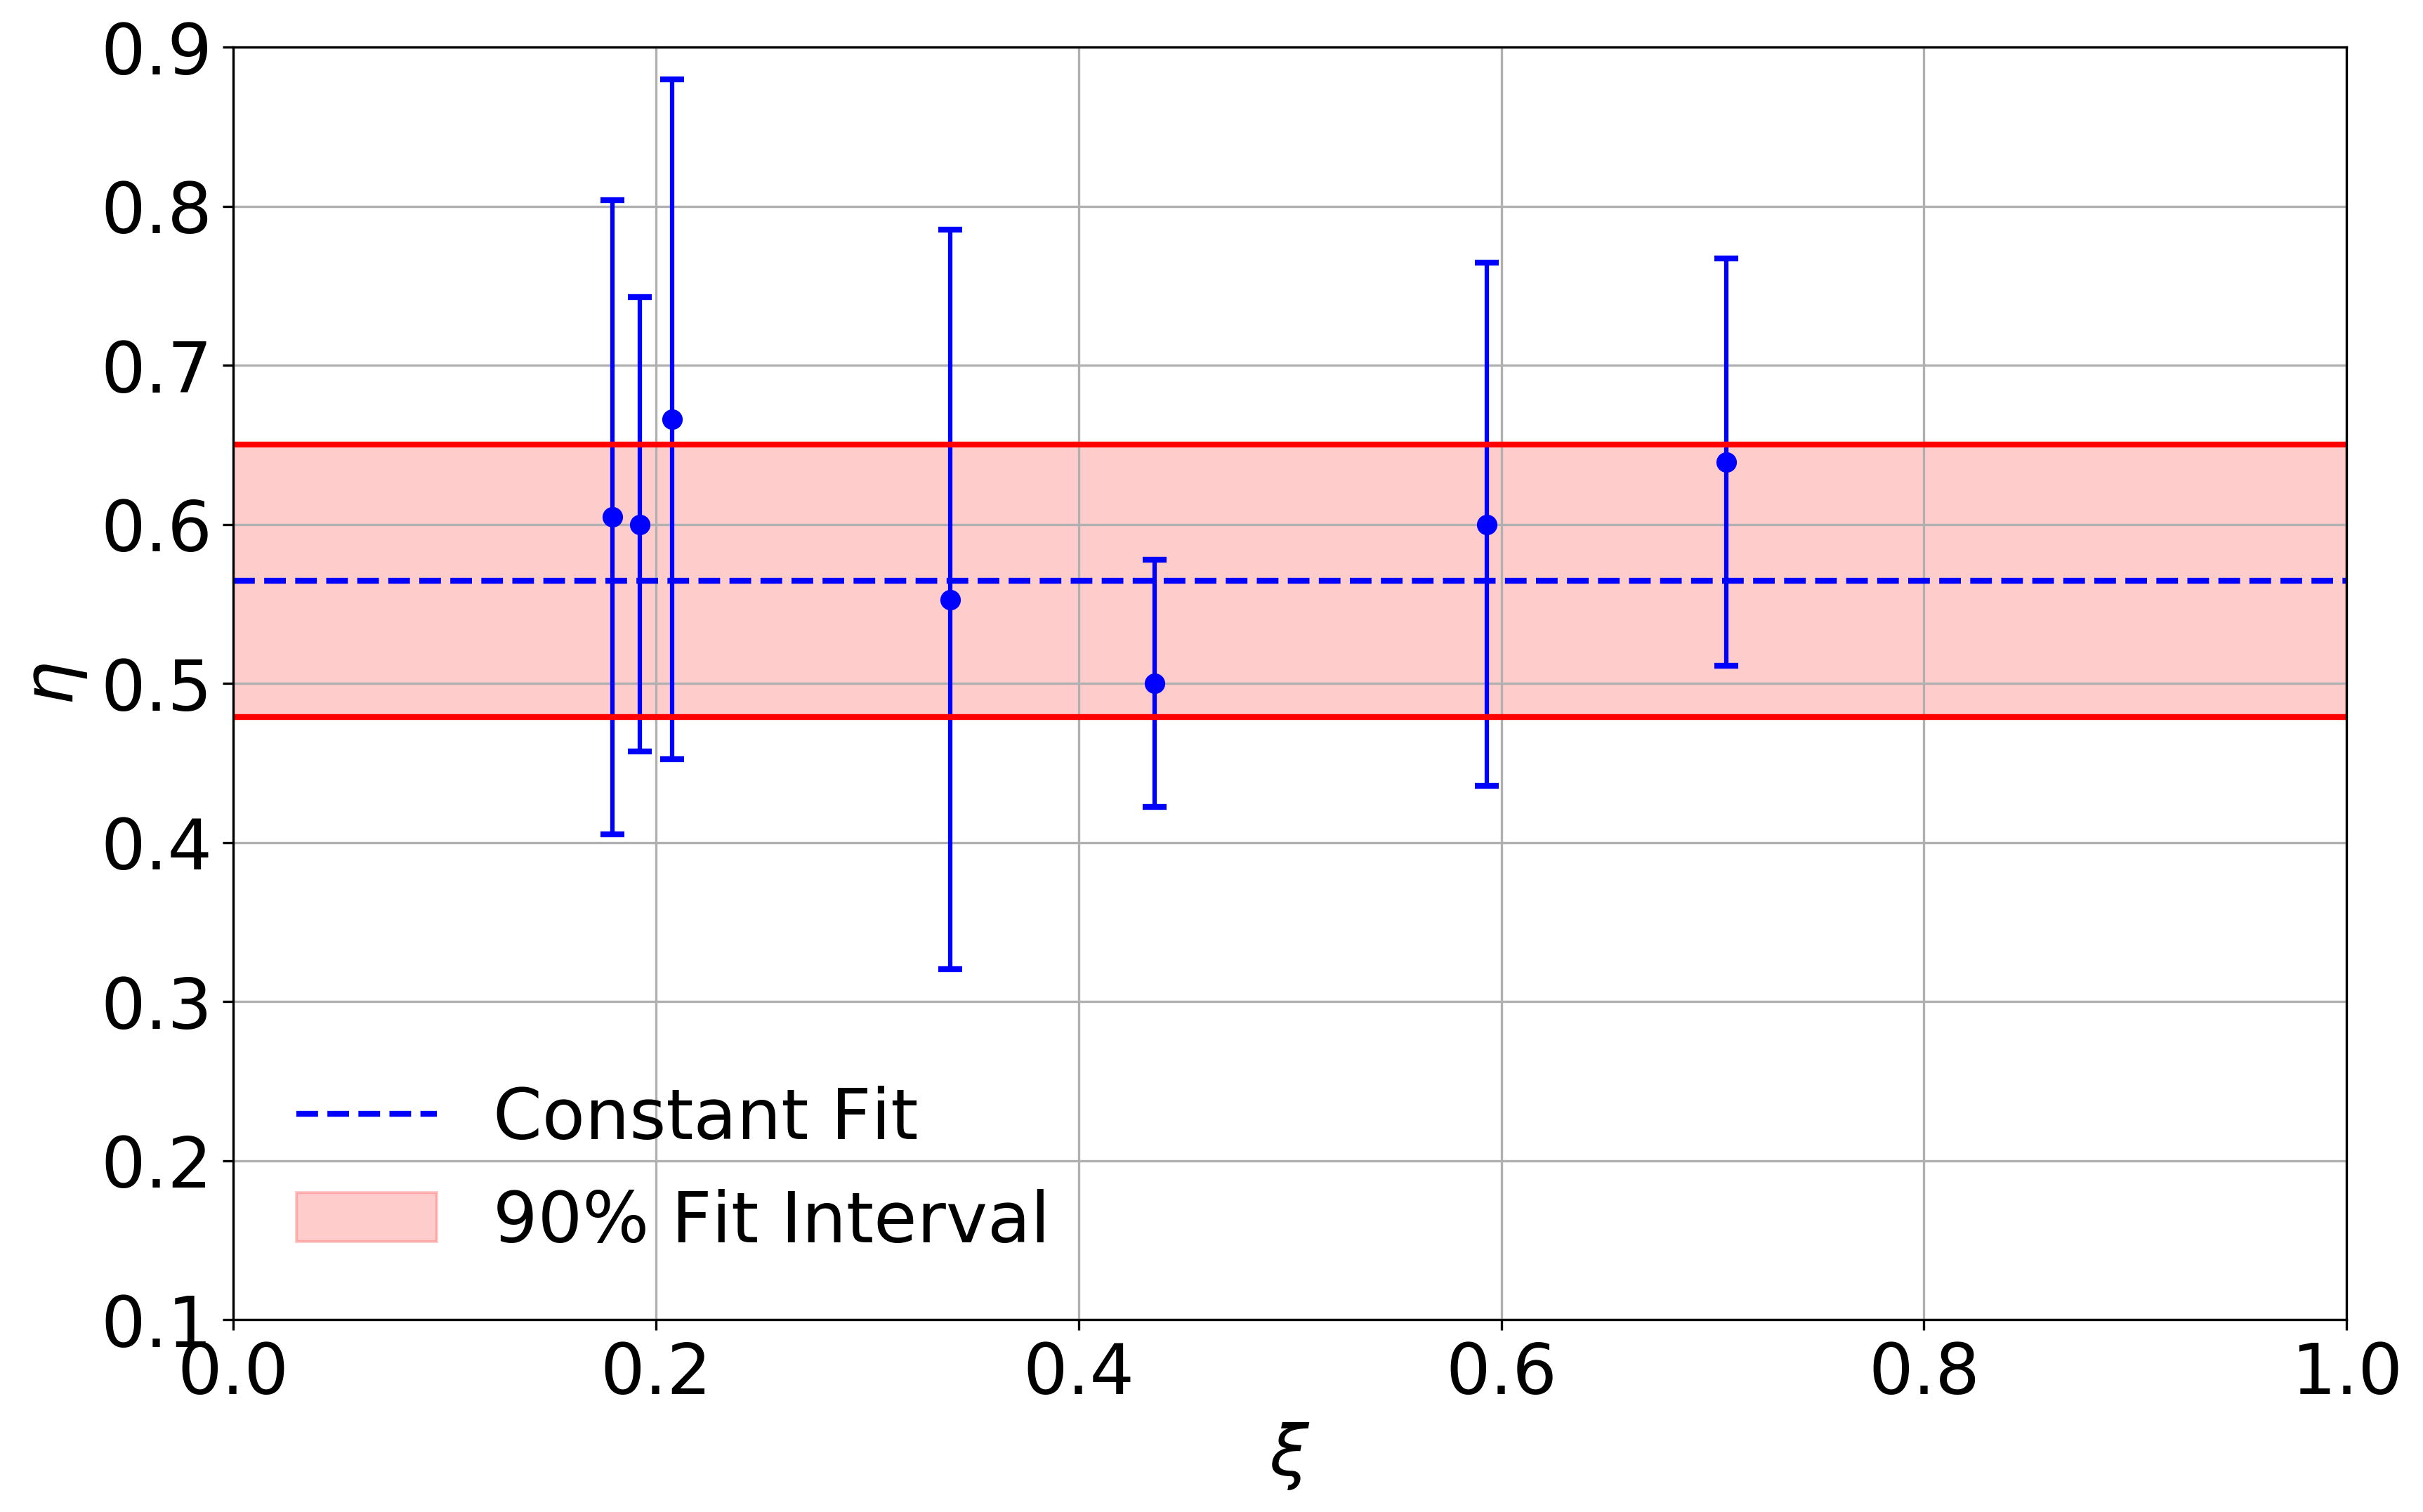
\includegraphics[width=0.8\textwidth]{images/Be_HOD_H_frac.png}
	\caption{}
	\label{}
\end{figure}

\section{Results and Discussion}

Because the \ce{HOD} sample also contains both \ce{H2O} and \ce{D2O}, the product \ce{BeOH+} ($m/z = 26$) has contributions of the reaction of the cation with \ce{H2O}, while \ce{BeOD+} ($m/z = 27$) has contributions from reactions with \ce{D2O}. The reactions of interest are:

\begin{align}
	\ce{Be+(^2S1/2) + H2O & -> BeOH+ + H} \\
	\ce{Be+(^2S1/2) + HOD & -> BeOD+ + H} \\
	\ce{& -> BeOH+ + D} \\
	\ce{Be+(^2S1/2) + D2O & -> BeOD+ + D}
\end{align}

Thus, the kinetics of the reagents and products are found from:

\begin{align}
	\dot{\ce{Be+}}(t) & = (k_1 \rho_1 + k_2 \rho_2 + k_3 \rho_3) \ce{Be+}(t) \\
	\dot{\ce{BeOH+}}(t) & = (k_1 \rho_1 + (1-\eta)k_2 \rho_2) \ce{Be+}(t) \\
	\dot{\ce{BeOD+}}(t) & = (k_3 \rho_3 + \eta k_2 \rho_2) \ce{Be+}(t)
\end{align}

where $k_i$ and $r_i$ are the rate coefficient and density for \ce{Be+} reacting \ce{H2O}, \ce{HOD}, and \ce{D2O} respectively. The branching ratio $\eta \equiv k_{\ce{BeOD+}}/(k_{\ce{BeOD+}} + k_{\ce{BeOH+}})$ is the fraction of \ce{BeOD+} produced from reactions (4.2) where $k_j$ is the rate coefficient of species $j$. Solutions to the rate equations (4.4)–(4.6) are parameterized by the density measurements of the water isotopologues taken from a RGA, and a least-squares fit is taken over data sets of integrated TOF mass spectra with shared fitting parameters $k_1$, $k_2$, $k_3$, and $\eta$. In order to extract the pure \ce{Be+(^2S1/2)} and \ce{Be+(^2P3/2)}-state branching ratios, the process shown in Fig. 1(A)–(C) was repeated at different P-state fractions. The results are shown in Fig. 1(D) along with a least-squares linear-fit (blue line). The vertical intercept of this fit gives $\eta_S = 0.56 \pm 0.03$ for the ground \ce{Be+(^2S1/2)} state reaction, while no conclusive dependence on P-state fractions is found within the confidence intervals. To further verify that our measurement is independent of reagent ratios, we repeated the measurement for different mixtures of \ce{HOD}, \ce{H2O}, and \ce{D2O}, as shown in Fig. 3. The branching ratio of \ce{BeOD+ + H} in reaction \ce{Be+ + HOD} (with 2\% \ce{Be+(^2P3/2)} state population) is consistent over different hydrogen fractions in the gas. The fraction of hydrogen atoms in the chamber ($\xi$) from all water isotopologues is defined by:

\begin{equation}
	\xi = \frac{2 \rho_{\ce{H2O}} + \rho_{\ce{HOD}}}{\rho_{\ce{H2O}} + \rho_{\ce{HOD}} + \rho_{\ce{D2O}}}
\end{equation}

Weighted averaging of the fitted values over different mixtures then gives $\eta = 0.58 \pm 0.14$, $frac{k_2}{k_1} = 0.8 \pm 0.9$, $\frac{k_3}{k_1} = 0.8 \pm 0.9$. Despite the large error bars on the relative rate coefficients, due to the significant covariance of the rate coefficients, $\eta$ is reasonably well determined. To further check our measurement of $\eta$, the process was repeated for shared fits with identical rate coefficients ($k1 = k2 = k3$) yielding $\eta = 0.57 \pm 0.07$. The calculated overall rate coefficients of the \ce{Be+ + D2O} and \ce{Be+ + HOD} reactions are $(2.29 \pm 0.05) \times 10^{-9}$ cm$^3$ molecule$^{-1}$ s$^{-1}$ and $(2.29 \pm 0.05) \times 10^{-9}$ cm$^3$ molecule$^{-1}$ s$^{-1}$, respectively, which are slightly larger than that ($(2.02 \pm 0.04) \times 10^{-9}$ cm$^3$ molecule$^{-1}$ s$^{-1}$)25 of the \ce{Be+ + H2O} reaction. The calculated $k_2/k_1$ and $k_3/k_1$ ratios are $1.13 \pm 0.04$ and $1.13 \pm 0.04$, which are consistent with experimental values of $0.8 \pm 0.9$ and $0.8 \pm 0.9$, respectively. The identical $k_2/k_1$ and $k_3/k_1$ ratios suggests the negligible isotopic effect in the thermal reaction probabilities of the \ce{Be+ + D2O} and \ce{Be+ + HOD} reactions. The branching ratio was determined using the QCT method for the \ce{Be+ + HOD} reaction. Specifically, the calculated branching fraction of \ce{Be+ + HOD} $(\eta)$ is $0.61 \pm 0.02$, which is in good agreement with experimental value $0.58 \pm 0.14$. The branching ratio of the two products (\ce{BeOD+} and \ce{BeOH+}) can be understood in terms of the PST model, which assumes complete energy randomization in the deep intermediate (\ce{BeHOD+}) well. In Fig. 4, the branching fraction for the \ce{BeOD+ + H} channel is plotted as a function of the collision energy, which shows very weak temperature dependence. At the specific collisional temperature 100 K, the fraction obtained by integrating the energy dependent branching ratio with a Boltzmann weight is 0.67, which is in reasonable agreement with the QCT results.

To shed more light onto the preference of the \ce{H + BeOD+} channel in the \ce{Be+ + HOD} reaction, we provide a further analysis of the two important factors in determining the branching ratio. In PST, the reactivity in a particular product channel is controlled by the availability of open states, which is in turn dictated by the rovibrational states of the corresponding product molecule above the exit barrier formed by the centrifugal potential. Due to the heavier deuterium, it is readily understood that there are more rovibrational states for \ce{BeOD+} than \ce{BeOH+}. However, the availability of open channels is also constrained by the orbital angular momentum ($l$), which erects a centrifugal barrier in both the reactant and product channels. The $l$-dependent centrifugal barrier is also isotope dependent, due to the difference in the reduced mass between the two products. The centrifugal barrier rises faster in the \ce{BeOD+ + H} channel than the \ce{BeOH+ + D} channel, due to the larger reduced mass of the latter. This is consistent with the fact that the branching fraction ($\eta$) of \ce{BeOD+ + H} channel becomes larger when the centrifugal barrier was not considered (shown in Fig. 4). These two factors have opposing effects on the branching ratio, but the higher density of states in the \ce{BeOD+} molecule dominates, at least at low energies. As a result, the \ce{H + BeOD+} product channel is strongly favored. The good agreement of the statistical model with both the experimental and QCT results in branching ratio suggests that the reaction is largely statistical. In addition, the DCSs of the \ce{Be+ + H2O/HOD/D2O} reactions calculated by the QCT method are shown in Fig. 5. It can be seen from the figure that the DCSs of all three reactions are roughly forward–backward symmetric, due to the long-lived intermediates formed in the reactions. The forward–backward symmetry in DCSs suggests the statistical nature of the reaction, which further validates the suitability of the PST model discussed above.

\section{Conclusion}

To summarize, chemical reactions between \ce{Be+(^2S1/2)} and \ce{HOD} have been investigated using an integrated ion trap and highresolution TOF-MS and ZPE corrected QCT calculations on an accurate global PES. Two product channels have been observed and the branching to \ce{BeOD+ + H} is accurately determined to be $0.58 \pm 0.14$. The experimental result is in good agreement with ZPE corrected QCT calculation result ($0.61 \pm 0.02$) as well as close to the statistical PST model (~0.67), which reveals that the branching to the two product channels is largely due to the availability of different open states in each channel. Since their rate coefficients deviate from the capture limit as reported in our earlier work, it is clear that the \ce{Be+(2S1/2) + H2O/D2O/HOD} reactions have a non-negligible non-statistical component. Interestingly, however, the good prediction of the branching ratio by the statistical model discussed above suggests that the formation of the products is largely statistical. This conclusion is further supported by the forward–backward symmetry of the calculated DCSs.

%\section{Notes}
%
%We mix "equal" amounts of \ce{H2O} and \ce{D2O} and leave it overnight to produce roughly 1:2:1 ratio of \ce{H2O}:\ce{HOD}:\ce{D2O} as roughly verified by the RGA. If we consider being a singular oxygen atom looking at a sea of \ce{H2O} and \ce{D2O}, it has a 1/4 probability of grabbing H or D twice. It then has a 1/2 chance of grabbing an H and D in either order, which gives us the 1:2:1 ratio.
%
%To generalize this, we can write the fraction of \ce{H2O} in the sample to be $\gamma$ and the \ce{D2O} to be $1-\gamma$. The probabilities of yielding any combination is then found quickly:
%
%\begin{align}
%	\ce{H2O}& = \gamma^2 \\
%	\ce{HOD}& = 2\gamma(1-\gamma) \\
%	\ce{D2O}& = (1-\gamma)^2
%\end{align}
%
%For the sake of readability, let (\ce{H2O}, \ce{HOD}, \ce{D2O}) be represented as (1, 2, 3) respectively.
%
%\begin{figure}[H]
%	\label{fig: mixture}
%	\centering
%	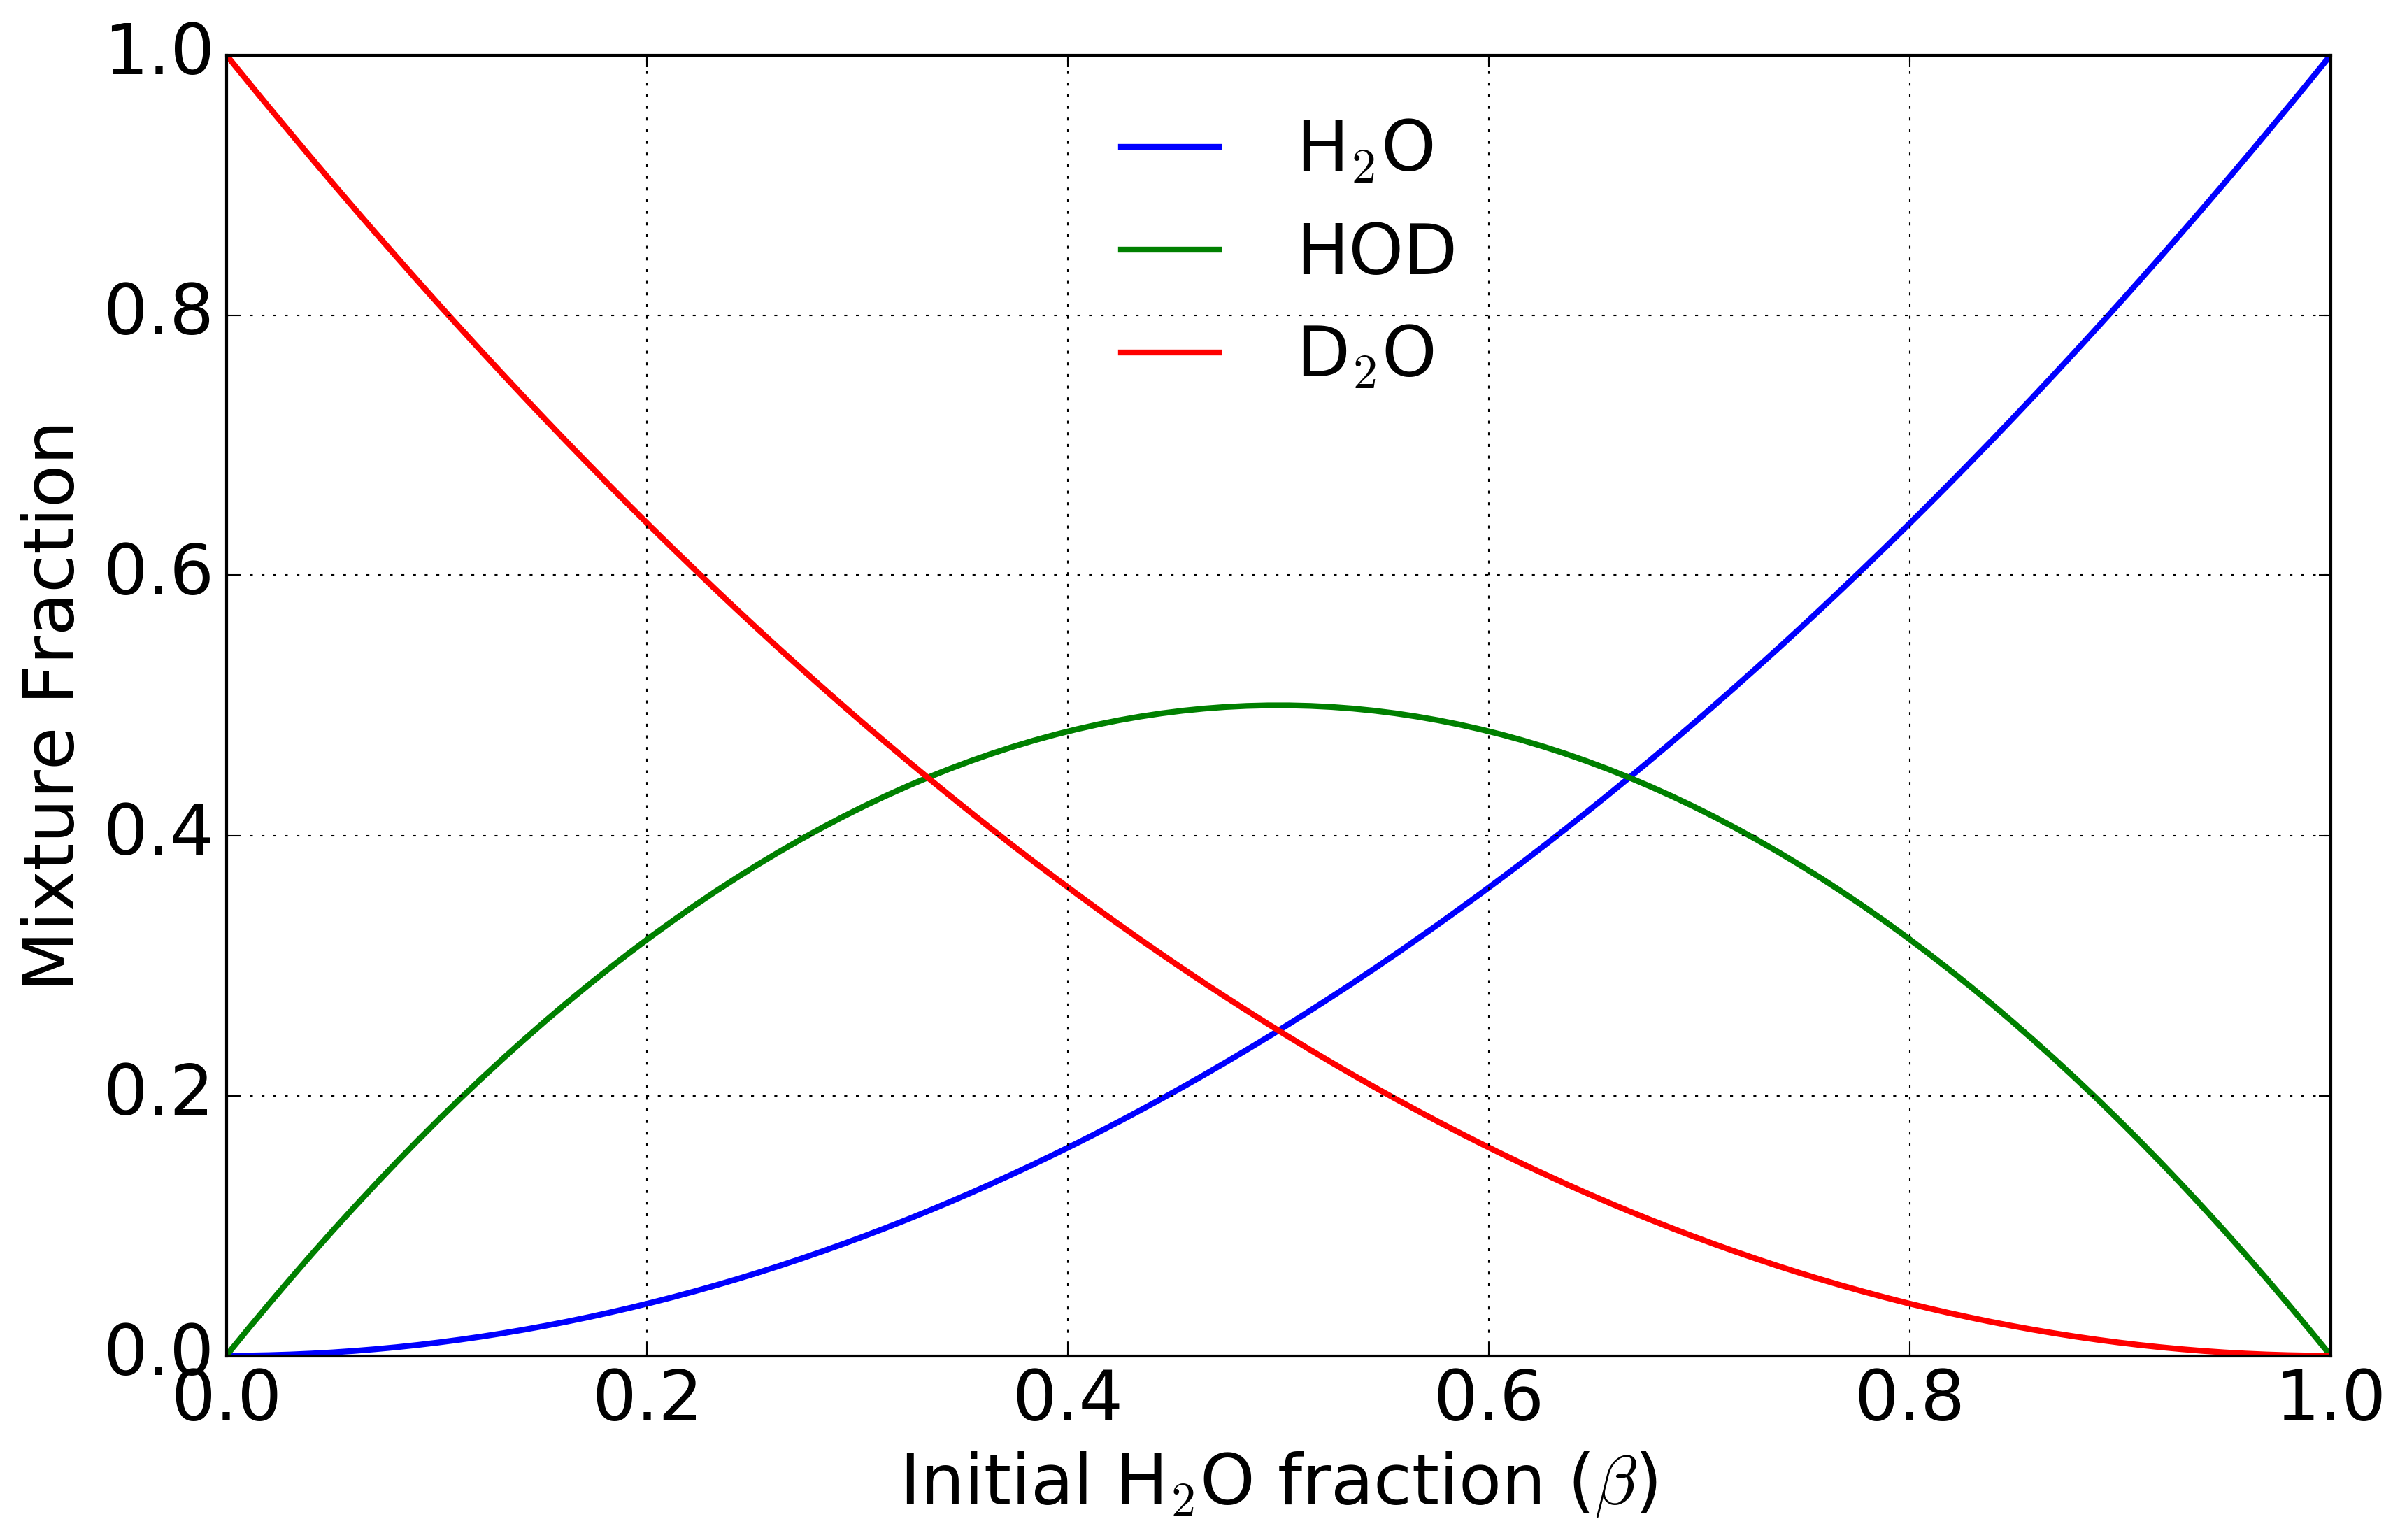
\includegraphics[width=0.8\textwidth]{images/Be_HOD_isotopologues.png}
%	\caption{}
%\end{figure}
%
%Reading water with an RGA causes some known fractionation, where the \ce{H2O} is broken into its constituents, including \ce{OH+} and \ce{O+}. We expect then to see a lower mass 18 peak than normal, to truly know what the ratios are, we have to calibrate the RGA ourselves.
%
%Possible fractionation pathways:
%
%\begin{align}
%	P'_{18} = & \alpha P_{\ce{H2O}} + \beta (\frac{P_{\ce{HOD}}}{2}+P_{\ce{D2O}}) \\
%	P'_{19} = & \alpha P_{\ce{HOD}} \\
%	P'_{20} = & \alpha P_{\ce{D2O}} \\
%	P'_{17} = & \beta (\frac{P_{\ce{HOD}}}{2} + P_{\ce{H2O}}) \\
%	P'_{16} = & \gamma (P_{\ce{H2O}} + P_{\ce{HOD}} + P_{\ce{D2O}}) \\
%	1 = & \alpha + \beta + \gamma
%\end{align}
%
%By solving this system of equations, we get 76.8\% of the real value as cited by the RGA program itself; this is also true for \ce{HOD} and \ce{D2O}. Of that lost 23.2\%, 18.4\% goes to \ce{OH+}, but for the isotopogues of \ce{HOD} and \ce{D2O}, we would need to consider which mass signal it will add to. No other mode of fractionation will contribute to the other water isotopologue peaks
%
%\begin{align}
%	P'_1 & = \alpha P_1 + \beta P_3 + \frac{\beta}{2} P_2 \\
%	P'_2 & = \alpha P_2 \\
%	P'_3 & = \alpha P_3
%\end{align}
%
%Where we let $\alpha = 0.744$ and $\beta=0.256$ per the SRS RGA software. Where P is the real pressure accounting for fractionation, and P' is the raw observed pressure value. Solving for the real pressure, we find:
%
%\begin{align}
%	P_1 & = \frac{1}{\alpha}\left(P'_1 - \frac{\beta}{\alpha}P'_3 - \frac{\beta}{2\alpha} P'_2\right) \\
%	P_2 & = \frac{P'_2}{\alpha} \\
%	P_3 & = \frac{P'_3}{\alpha}
%\end{align}
%
%\section{\ce{Be+ + HOD} branching ratio}
%
%Now that we can characterize the pressures in the chamber more accurately, we then consider the possible reactions between the \ce{Be+} and water isotopologues:
%
%\begin{align}
%	\ce{Be+ + H2O & -> BeOH+ + H} \\
%	\ce{Be+ + HOD & -> BeOH+ + H} \label{eq: beoh} \\
%	\ce{& -> BeOD+ + H} \label{eq: beod} \\
%	\ce{Be^+ + D2O & -> BeOD+ + D}
%\end{align}
%
%Which can then be written as a system of differential equations.
%
%\begin{align}
%	\dot{Be}(t) & = -(k_1\rho_1+k_2\rho_2+k_3\rho_3)Be(t) \\
%	\dot{BeOH}(t) & = (k_1\rho_1+(1-\eta)k_2\rho_2)Be(t) \\
%	\dot{BeOD}(t) & = (k_3\rho_3+\eta k_2\rho_2)Be(t)
%\end{align}
%
%We are interested in reactions \ref{eq: beoh} and \ref{eq: beod} and the ratio between the two ($\eta$), which is not directly found from the ratio of the production rates of the two ions. Since this is a ratio, we don't need to concern ourselves with calculating the density ($\rho$), the RGA pressure is fine.
%
%\begin{align}
%	\beta \equiv \frac{\dot{BeOD}}{\dot{BeOH}} & = \frac{k_3P_3 + \eta k_2P_2}{k_1P_1 + (1-\eta)k_2P_2} \\
%	\eta & = \frac{\beta(k_1P_1 + k_2P_2)-k_3P_3}{k_2P_2(1+\beta)}
%\end{align}
%
%The theorists found that the statistical value of the reaction is around 3, but with dynamics, tends towards $\frac{\eta}{1-\eta} = 1.7$ or $\eta=0.63$ for Be$^+$(S).
